\section{Ideale Quantengase}
\subsection{Quantenmachanik nicht-wechselwirkender Teilchen}
\begin{tabbing}
\hspace{4em} \= \hspace{4em} \= \kill
Hamiltonoperator: \quad $H = \sum\limits_{j=1}^{N} H^{(j)}$ \quad (keine WW-Terme)\\
Energie-Eigenzustände $\Psi_E$: \quad $H \, \Psi_E = E \, \Psi_E$\\
können als Produktzustände von Einteilchenzuständen $\Phi_{\alpha}^{(j)}$ konstruiert werden:\\
\> $\Psi_E = \Psi_E\left(x^{(1)},\dots, x^{(N)}\right) = \Phi_{\alpha(1)}^{(1)}\left(x^{(1)}\right) \dots \Phi_{\alpha(N)}^{(N)}\left(x^{(N)}\right)$\\
\> $x^{(1)}$: Koordinaten und / oder Spin von Teilchen 1\\
\> $H^{(j)}\Phi_{\alpha}^{(j)} = \varepsilon_{\alpha}^{(j)} \Phi_{\alpha}^{(j)}$\\
\> $E = \sum\limits_{j=1}^{N} \varepsilon_{\alpha(j)}^{(j)}$\\
Kanonisches Ensemble:\\
\> $ Z = \sum\limits_{\alpha_1}\dots \sum\limits_{\alpha_N} \exp \left(-\beta \left(\varepsilon_{\alpha_1}^{(1)} + \dots + \varepsilon_{\alpha_N}^{(N)}\right)\right)$\\
\> $ Z = Z^{(1)} \dots Z^{(N)}$\\
\> $Z^{(j)}$: Zustandssumme von Teilchen j\\
Identische Teilchen:\\
\> $Z^{(1)} = \dots = Z^{(N)}$\\
$\rightarrow$ \> $Z = \left(Z^{(1)}\right)^N$\quad (nur richtig für \underline{unterscheidbare} Teilchen)\\
\uwave{Beispiel}: Gas im Volumen $V= L^3$, Periodische Randbedingungen\\
\> $\Phi_{\alpha}\left(\vec{q}\right) = \frac{1}{\sqrt{V}} \exp \left(i \vec{p}_{\alpha}\cdot \vec{q}\right)$\\
\>$\vec{p}_{\alpha} = \left(p_{\alpha,1}, p_{\alpha,2}, p_{\alpha,3}\right)^T$\\
\> $p_{\alpha,j} = \frac{2\,\pi \,\hbar}{L}\cdot \nu_{\alpha,j}$
($\nu_{\alpha,j} \in \mathbb{Z}$)\\
\>Energie: $\varepsilon_{\alpha} = \frac{\vec{p}_{\alpha}^2}{2\, m}$\\
Identische Quantenteilchen sind \underline{ununterscheidbar}. Es gibt 2 Arten:\\
-- \underline{ Fermionen}, \> \>$\Phi(\dots,x,\dots,y,\dots) = - \Phi(\dots,y,\dots,x,\dots)$\\
  \>\> (antisymmetrisch unter Teilchenvertauschung)\\
-- \underline{Bosonen}, \> \> $\Phi(\dots,x,\dots,y,\dots) = \Phi(\dots,y,\dots,x,\dots)$\\
  \>\> (symmetrisch)\\
$\rightarrow$ \> Produktzustände im Allgemeinen nicht richtig, Zahl der Zustände stark reduziert.\\
$\rightarrow$ \> Wir benötigen \underline{andere Zählweise}\\
Erlaubte Zustände sind (anti-)symmetrische Linearkombinationen von Produktzuständen:\\
\>$\Phi_{\alpha_1} \otimes \dots \otimes \Phi_{\alpha_N} = \Phi_{\alpha_1}\dots \Phi_{\alpha_N}$\\
\> $\Psi = \mathcal{N} \sum\limits_{\pi}\,P_{\pi}\left[\Phi_{\alpha_1}\dots \Phi_{\alpha_N}\right]$ \quad (Bosonen, vollständig symmetrisch)\\
\> $\Psi = \mathcal{N} \sum\limits_{\pi}\,(-1)^{\pi}\,P_{\pi}\left[\Phi_{\alpha_1}\dots \Phi_{\alpha_N}\right]$ \quad (Fermionen, vollständig antisymmetrisch)\\
\> $\mathcal{N}$: Normierungsfaktor (für Fermionen / Bosonen verschieden)\\
\> $\pi$: Permutation\\
\> Signum: $(-1)^{\pi} = \sigma(\pi) = \left\{ \begin{array}{r@{\quad : \quad} l }1 & \text{gerade Permutation}\\ -1 & \text{ungerade Permutation}\\\end{array}\right.$\\
Zustand ist vollständig angegeben durch die \underline{Besetzungszahlen} $n_{\alpha}$,\\
das heißt Zahl der Teilchen im Einteilchenzustand $\Phi_{\alpha}$.\\
\> Fermionen: $n_{\alpha} \in \{0,1\}$\\
\> Bosonen: $n_{\alpha} \in \mathbb{N}$\\
\uwave{Beispiel}: 2 Teilchen, 2 Einzelteilchenzustände
\end{tabbing}

\begin{table}[H]
\begin{tabular}{c c c c c}
  \underline{Klassisch} & & \underline{Fermionen} & & \underline{Bosonen}\\\footnotesize
  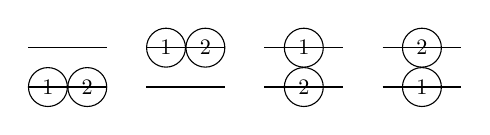
\begin{tikzpicture}[scale = 0.5, every node/.style = {minimum size = 1.5em, scale = 0.8}]
    \path[draw] (0,0) to (2,0);
    \path[draw] (0,-1) to (2,-1);
    \node[draw,circle] at (0.5,-1) {1};
    \node[draw,circle] at (1.5,-1) {2};

    \path[draw] (3,0) to (5,0);
    \path[draw] (3,-1) to (5,-1);
    \node[draw,circle] at (3.5,0) {1};
    \node[draw,circle] at (4.5,0) {2};

    \path[draw] (6,0) to (8,0);
    \path[draw] (6,-1) to (8,-1);
    \node[draw,circle] at (7,0) {1};
    \node[draw,circle] at (7,-1) {2};

    \path[draw] (9,0) to (11,0);
    \path[draw] (9,-1) to (11,-1);
    \node[draw,circle] at (10,-1) {1};
    \node[draw,circle] at (10,0) {2};
  \end{tikzpicture} &\hspace*{1cm}&
  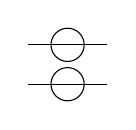
\begin{tikzpicture}[scale = 0.5, every node/.style = {minimum size = 1.5em, scale = 0.8}]
    \path[draw] (0,0) to (2,0);
    \path[draw] (0,-1) to (2,-1);
    \node[draw,circle] at (1,-1) {};
    \node[draw,circle] at (1,0) {};
  \end{tikzpicture} &\hspace*{1cm}&
  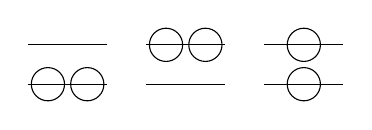
\begin{tikzpicture}[scale = 0.5, every node/.style = {minimum size = 1.5em, scale = 0.8}]
    \path[draw] (0,0) to (2,0);
    \path[draw] (0,-1) to (2,-1);
    \node[draw,circle] at (0.5,-1) {};
    \node[draw,circle] at (1.5,-1) {};

    \path[draw] (3,0) to (5,0);
    \path[draw] (3,-1) to (5,-1);
    \node[draw,circle] at (3.5,0) {};
    \node[draw,circle] at (4.5,0) {};

    \path[draw] (6,0) to (8,0);
    \path[draw] (6,-1) to (8,-1);
    \node[draw,circle] at (7,0) {};
    \node[draw,circle] at (7,-1) {};
  \end{tikzpicture}\\\normalfont
  4 Zustände & & 1 Zustand & & 3 Zustände \\
\end{tabular}
\end{table}
\begin{tabbing}
\hspace{4em} \= \hspace{4em} \= \kill
Der Korrekturfaktor $\frac{1}{N!}$ (siehe Gibbs-Paradoxon) liefert eine Näherung,\\
die für kleine besetzungszahlen gut ist ($T \to \infty$).\\
Hier: $\frac{1}{N!}\cdot 2^N = \frac{1}{2!}2^2 = 2$ Zustände (liegt zwischen fermionischem/ bosonischem Fall)\\

\underline{Struktur des Hilbertraums}\\
Für 2 Teilchen: nur 2 mögliche Permutationen\\
\> $\pi_1 = (1,2)$ (neutrales Element), $\pi_2 = (2,1)$ (Transposition),\\
\> bilden \underline{Permutationsgruppe} $S_2 = \left\{(1,2),(2,1)\right\}$\\
Für Zweiniveausysteme: $\mathcal{H} = \mathbb{C}^2 \otimes \mathbb{C}^2$,\\
\> Basiszustände $\vec{e}_{j,k} := \vec{e}_j\otimes\vec{e}_k$\\
\> mit $\vec{e}_1 = \left(1, 0\right)$, $\vec{e}_2 = \left(0, 1\right)$\\
$\mathcal{H}$ zerfällt in \underline{symmetrischen Unterraum} $\mathcal{H}_-$ und \underline{antisymmetrischen Unterraum} $\mathcal{H}_+$:\\
\> $\mathcal{H}_- = \left\langle\left(\vec{e}_{1,2} - \vec{e}_{2,1}\right)/\sqrt{2}\right\rangle_{\mathbb{C}}$\\
\> $\mathcal{H}_+ = \left\langle \vec{e}_{2,2}, \vec{e}_{1,1}, \left(\vec{e}_{1,2} + \vec{e}_{2,1}\right)/\sqrt{2}\right\rangle_{\mathbb{C}}$\\
\> $\langle\cdot\rangle_{\mathbb{C}}$: Span bzw. lineare Hülle\\
Das soll heißen, es gilt:\\
\> $P_{\pi} (\Psi) = (-1)^{\pi} \Psi \;\; \forall\,\Psi\!\in\!\mathcal{H}_-$\\
\> $P_{\pi} (\Psi) = \Psi \;\; \forall\,\Psi\!\in\!\mathcal{H}_+$\\
Für mehr als zwei Teilchen gibt es \underline{weitere Unterräume} außer $\mathcal{H}_-$ und $\mathcal{H}_+$
\end{tabbing}


\subsection{Großkanonische Behandlung, Besetzungsstatistik}
\begin{tabbing}
\hspace{4em} \= \hspace{4em} \= \kill
Besetzungszahlen: $n_j$, Vielteilchenzustand: $\nu = \left\{ n_1,n_2, \dots\right\}$\\
\> Energie: $E_{\nu} = \sum\limits_{j} n_j \varepsilon_j$,\\
\> Teilchenzahl: $N_{\nu} = \sum\limits_{j} n_{j}$\\
\> Besetzungswahrscheinlichkeiten: $p_{\nu} = \frac{1}{Z} \exp \left(-\beta\left(E_{\nu}- \mu N_{\nu}\right)\right)$\\
\> $Z = \sum\limits_{\nu} \exp \left(-\beta\left(E_{\nu} - \mu N_{\nu}\right)\right)$: Großkanonische Zustandssumme\\
Bei unterscheidbaren Teilchen ist $Z = \sum\limits_{\{n_j\}}\frac{\left(\sum_j n_j\right)!}{\prod_j\left(n_j!\right)}\exp\left(-\beta\sum_j n_j \left(\varepsilon_j - \mu\right)\right)$\\
$Z$\> $= \sum\limits_{n_1}\sum\limits_{n_2}\dots \exp \left(-\beta \sum_{j} n_{j} \left(\varepsilon_j - \mu\right)\right) $\\
\>$=\sum\limits_{n_1} \exp \left(-\beta n_1 \left(\varepsilon_1 - \mu\right)\right) \cdot \sum\limits_{n_2} \exp \left(-\beta n_2 \left(\varepsilon_2 - \mu\right)\right) \dots $\\
$\rightarrow$ \> $Z = \prod\limits_j Z_j$\\
\> $Z_j = \sum\limits_j \exp - \beta n_j \left(\varepsilon_j - \mu\right)$\\
Formal wie ein System mit unterscheidbaren Subsystemen (=Einzelteilchenzustände).\\
\>Besetzung des Einteilchenzustands j: $p_j(n) = \frac{1}{Z_j} \exp - \beta n \left(\varepsilon_j - \mu\right)$\\
\>Großkanonisches Potential (Landau-Potential): $\Phi = -k_B T \ln Z$\\
$\rightarrow$\> $\Phi = \sum\limits_j \Phi_j$\\
\> $\Phi_j = -k_B T \ln Z_j$\\


\underline{Fermi-Dirac-Statistik}\\
$n_j = 0,1$\\
$\rightarrow$\> $Z_j = \sum\limits_{n = 0}^{1}\exp \beta n \left(\mu - \varepsilon_j\right) = 1 + \exp \beta n \left(\mu - \varepsilon_j\right)$, $\Phi_j = - k_B T \ln \left(1 + e^{\beta (\mu - \varepsilon_j)}\right)$\\
\>Wahrscheinlichkeit, dass Teilchen in Zustand j: $p_j(n) = \frac{\exp \beta n \left(\mu - \varepsilon_j \right)}{1+ \exp \beta (\mu - \varepsilon_j)}$\\
\>Mittlere Teilchenzahl in Zustand j: \fbox{$\langle n_j \rangle = p_j(1) = \frac{1}{1+ \exp \beta (\varepsilon_j - \mu)}$}\\
\>$E = \langle E \rangle = \sum\limits_j \varepsilon_j \langle n_j \rangle$\\
\> $N = \langle N \rangle = \sum\limits_j \langle n_j\rangle$\\
Möglichkeit $\beta$ ,$\mu$ zu bestimmen aus N, E beziehungsweise umgekehrt.\\


\underline{Bose-Einstein-Statistik}\\
$n_j = 0,1,2,\dots$\\
$\rightarrow$\> $Z_j = \sum\limits_{n = 0}^{\infty} \exp \beta n (\mu - \varepsilon_j)$ konvergiert für $\exp \beta (\mu - \varepsilon_j) < 1$ das heißt, $\mu < \varepsilon_j$\\
$\rightarrow$ \> Es muss gelten $\mu < \varepsilon_0$ mit Grundzustandsenergie $\varepsilon_0$.\\
(Erklärung: Nach Hinzufügen eines Teilchens muss Energie reduziert werden (Annahme: $\varepsilon_0 = 0$),\\
\> um Entropie konstant zu halten, $\mu = \left(\frac{\partial E}{\partial N}\right)_{S,V}$.)\\
$\rightarrow$\> $Z_j = \frac{1}{1 - \exp \beta (\mu - \varepsilon_j)}$\\
\> $\Phi_j = k_B T \ln \left(1 - \exp \beta (\mu - \varepsilon_j)\right)$\\
\>$p_j(n) = \exp \left(\beta n (\mu - \varepsilon_j)\right)\left(1 - e^{\beta (\mu - \varepsilon_j)}\right)$\\
\>$\langle n_j \rangle = \sum_n n \exp \left(\beta n(\mu - \varepsilon_j)\right)\left(1-e^{\beta(\mu - \varepsilon_j)}\right)$ (alternativ $\langle n_j\rangle = -\left(\frac{\partial \Phi_j}{\partial \mu}\right)_{T,V}$)\\
Summe: $\frac{\partial}{\partial \alpha}\sum\limits_n e^{n \alpha} = \frac{\partial}{\partial \alpha} \frac{1}{1 - e^{\alpha}} = \frac{e^{\alpha}}{(1 - e^{\alpha})^2}$, mit $\alpha = \beta (\mu - \varepsilon_j)$\\
$\rightarrow$\> $\langle n_j \rangle = \frac{e^{\beta(\mu - \varepsilon_j)}}{1 - e^{\beta (\mu - \varepsilon_j)}}$\\
$\rightarrow$\> \fbox{$\langle n_j \rangle = \frac{1}{e^{\beta (\varepsilon_j - \mu)} - 1}$}\\


\underline{Klassischer Grenzfall} (\glqq \underline{nichtentartetes Gas}\grqq)\\
Falls $\mu \ll\varepsilon_j$, $e^{\beta(\varepsilon_j - \mu)} \gg 1$, dann $\langle n_j \rangle \approx e^{\beta (\mu - \varepsilon_j)}\ll 1$\\
$\Phi_j = \stackrel[\scriptstyle{BE}]{\scriptstyle{FD}}{\mp} k_B T \ln\left(1\pm e^{\beta(\mu - \varepsilon_j)}\right)\approx - k_B T e^{\beta (\mu - \varepsilon_j)}\approx - k_B T \langle n_j \rangle$\\
Näherung: $\ln (1\pm x)\approx \pm x$\\
$\rightarrow$\> $\Phi = \sum\limits_j \Phi_j = - k_B T N$\\
Euler-Theorem für homogenes System: $E = T S - p V + \mu N$\\
$\rightarrow$\> $\Phi = E - T S - \mu N = - p V$\\
ergibt: \> \fbox{$p V = N k_B T$} (\underline{thermische Zustandsgleichung})\\
\uwave{Beachte}: Wir haben nicht verwendet, welche Form $\varepsilon_j$ hat.\\
\uwave{Beispiel}:
\end{tabbing}
\setlength{\tabcolsep}{2em}
\begin{table}[H]
  \centering
  \begin{tabular}{c c c}
  $\varepsilon_j = \frac{\vec{p}_j^2}{2 m}$ & $\varepsilon_j = \frac{\vec{p}_j^2}{2 m} + \frac{\hbar^2}{2 I}l (l+1)$ & $\varepsilon_j^2 = (mc^2)^2 + c^2\vec{p}_j^2$\\
  Freies Teilchen & Moleküle mit Drehimpuls & relativistische Teilchen \\
  \end{tabular}
\end{table}
\setlength{\tabcolsep}{1pt}
\begin{tabbing}
\hspace{4em} \= \hspace{4em} \= \kill
Betrachte den klassischen Grenzfall für $\varepsilon_j = \frac{\vec{p}_j^2}{2 m}$:\\
$N = \sum\limits_j \langle n_j \rangle = e^{\beta\mu}\sum\limits_j e^{-\beta\varepsilon_j} = e^{\beta\mu}\int\limits\frac{V}{h^3}e^{-\beta\frac{\vec{p}^2}{2 m}}\cdot g \dd{} ^3 \vec{p} = e^{\beta\mu}\cdot\frac{g V}{h^3}\cdot \sqrt{2 \pi m k_B T}^3$\\
Entartungsgrad: $g = 2 s + 1$\\
$\rightarrow$\> \fbox{$e^{\frac{\mu}{k_B T}} = \frac{N}{g V}\cdot \Lambda^3$} (\underline{Fugazität}) mit \fbox{$\Lambda = \frac{h}{\sqrt{2 \pi m k_B T}}$} $=$ \underline{thermische de Broglie-Wellenlänge}\\
Bedingung für klassisches Gas: $e^{\frac{\mu}{k_B T}}\ll 1$, das heißt $\Lambda^3 \ll \frac{V}{N}$ (Wellenlänge $\ll$ Teilchenabstand)\\
$\rightarrow$\> $\mu = k_B T \ln\left(\frac{N}{g V}\cdot\Lambda^3\right) = k_B T \ln\left(\frac{p}{g k_B T}\cdot\Lambda^3\right)$, \fbox{$\Phi = -\frac{g V}{\Lambda^3}k_B T e^{\frac{\mu}{k_B T}}$} (da $\Phi = -k_B T N$)\\
Freie Enthalpie: $G = \mu N = N k_B T \ln \frac{p \Lambda^3}{g k_B T}$\\
Herleitung der \underline{kalorischen Zustandsgleichung} (Zusammenhang zwischen E und T,V,N):\\
Freie Energie: $F = G -p V = N k_B T \ln \left(\frac{N}{g V} \Lambda^3\right) - N k_B T$\\
\> $\dd F = -S \dd T -p \dd V + \mu \dd N$\\
$\rightarrow$\> $S = -\left(\frac{\partial F}{\partial T}\right)_{V,N} = - N k_B \ln\left(\frac{N \Lambda^3}{g V}\right) - N k_B T \left(-\frac{3}{2}\right)\frac{1}{T} + N k_B = - N k_B \ln\left(\frac{N \Lambda^3}{g V}\right) + \frac{5}{2} N k_B$\\
$\rightarrow$\> \fbox{$E = F + T S = \frac{3}{2}N k_B T = \frac{3}{2} p V$}
\end{tabbing}


\subsection{Schwach entartetes Gas}
\begin{tabbing}
\hspace{4em} \= \hspace{5em} \= \kill
Betrachte den Fall $\langle n_j \rangle \ll 1$, aber mit erster Quantenkorrektur:\\
$\Phi = \stackrel[\scriptstyle{BE}]{\scriptstyle{FD}}{\mp} k_B T \ln\left(1\pm e^{\beta (\mu - \varepsilon_j)}\right)\approx - k_B T \sum\limits_j e^{\beta(\mu - \varepsilon_j)}\mp \left[-\frac{k_B T}{2}\sum\limits_j e^{2 \beta (\mu - \varepsilon_j)} \right]$\\
$\Phi \approx \Phi_{klass}(T,V,\mu) \mp \Phi_{klass}(\frac{T}{2},V,\mu) = -\frac{g V k_B T}{\Lambda^3}e^{\frac{\mu}{k_B T}}\mp -\frac{g V k_B \frac{T}{2}}{\Lambda^3\cdot2^{\frac{3}{2}}} e^{2\frac{\mu}{k_B T}}$\\
$\rightarrow$\> $\Phi(T,V,\mu) = \Phi_{klass}(T,V,\mu)\cdot\left[1\mp\frac{e^{\frac{\mu}{k_B T}}}{2^{\frac{5}{2}}}\right]$\\
Suche Modifikation der thermischen Zustandsgleichung $\rightarrow$ berechne Druck:\\
\> $p = -\left(\frac{\partial \Phi}{\partial V}\right)_{T,\mu} = \frac{g k_B T}{\Lambda^3} e^{\frac{\mu}{k_B T}}\cdot \left[1\mp\frac{e^{\mu/k_B T}}{2^{5/2}}\right]$\\
Wir möchten p durch T,V,N ausdrücken $\rightarrow$ drücke $\mu$ durch N aus:\\
\> $N = -\frac{\partial \Phi}{\partial \mu} = \frac{g V}{\Lambda^3}e^{\frac{\mu}{k_B T}} \mp \frac{g V}{\Lambda^3} \frac{1}{2^{5/2}}e^{2\frac{\mu}{k_B T}}$ $\rightarrow$ $e^{\frac{\mu}{k_B T}} \mp \frac{1}{2^{5/2}}\left(e^{\frac{\mu}{k_B T}}\right)^2 = \frac{N \Lambda^3}{g V}$\\
$e^{\frac{\mu}{k_B T}} \ll 1$ $\rightarrow$ $e^{\frac{\mu}{k_B T}} \approx \frac{N \Lambda^3}{g V}$ $\rightarrow$ nächste Korrektur: $e^{\frac{\mu}{k_B T}} = \frac{N \Lambda^3}{g V} \left(1 \pm \frac{1}{2^{3/2}}\frac{N \Lambda^3}{g V}\right)$\\
Einsetzen in p: $p \approx \frac{g k_B T}{\Lambda^3}\frac{n \Lambda^3}{g V}\left(1 \pm \frac{1}{2^{3/2}}\frac{N \Lambda^3}{g V}\right)\cdot \left[1 \mp \frac{1}{2^{5/2}}\frac{N \Lambda^3}{g V}\right]$\\
$\rightarrow$\> $p V = N k_B T \cdot \left(1 \pm \frac{1}{2^{3/2}}\frac{N \Lambda^3}{g V} \mp \frac{1}{2^{5/2}}\frac{N \Lambda^3}{g V} + \dots\right)$\\
$\rightarrow$\> \fbox{$p V = N k_B T\cdot\left(1 \pm \frac{1}{2^{5/2}}\frac{N \Lambda^3}{g V}\right)$}\\
\glqq $+$\grqq: \> Fermionen,\> $p > p_{klass}$, \underline{repulsive Austauschkräfte}\\
\glqq $-$\grqq: \> Bosonen,\> $p < p_{klass}$, \underline{attraktive Austauschkräfte}
\end{tabbing}


\subsection{Entartetes Gas}
\begin{tabbing}
\hspace{4em} \= \hspace{4em} \= \kill
Für einige Zustände sei $\langle n_j \rangle \ll 1$ stark verletzt. Wir suchen:\\
$\Phi = \mp k_B T \sum\limits_j \ln \left(1\pm e^{\beta(\mu - \varepsilon_j)}\right)$ (da $\Phi$ die Berechnung thermodynamischer Eigenschaften erlaubt)\\
Betrachte Teilchen mit $\varepsilon_j = \frac{\vec{p}^2}{2 m}$, zusätzlich mit Spinfreiheitsgrad.\\
$\sum\limits_j (\dots) = \int \frac{V}{h^3} \dd{}^3p\cdot g\cdot (\dots )$ mit $g = 2s + 1= \left\{\begin{array}{r@{\quad : \quad} l} 1 & \text{Spin } s=0\\ 2 & \text{Spin } s = \frac{1}{2}\\ . & \dots\dots\dots \end{array}\right.$\\
$\varepsilon = \frac{p^2}{2 m}$ $\rightarrow$ $\dd{p} = \sqrt{2 m}\frac{1}{2\sqrt{\varepsilon}}\dd{\varepsilon}$\\
$\sum\limits_j (\dots) = \frac{g V}{h^3} \int\limits_0^{\infty} 4\pi 2 m \varepsilon \sqrt{2 m}\frac{1}{2 \sqrt{\varepsilon}}\dd{\varepsilon}(\dots) = \frac{2 \pi g V}{h^3} (2 m)^{3/2}\int\limits_0^{\infty}\sqrt{\varepsilon}\dd{\varepsilon}(\dots)=:\int\limits_0^{\infty}\rho(\varepsilon)\dd{\varepsilon}(\dots)$\\
Mit \underline{Zustandsdichte} $\rho(\varepsilon) \sim \sqrt{\varepsilon}$
\end{tabbing}
\begin{figure}[H]
  \centering
  \begin{tikzpicture}[every node/.style = {draw = none, fill = none,scale = 0.8},domain=0:2]
    \draw[->] (0,-0.15) to (0,3);
    \draw[->] (-0.15,0) to (5,0);
    \node[anchor=west] at (0,3.25) {$\rho(\varepsilon)$};
    \node at (5.5,0) {$\varepsilon$};
    \draw[thick] plot ({\x^2},\x);
  \end{tikzpicture}
\end{figure}
\begin{tabbing}
\hspace{4em} \= \hspace{4em} \= \kill
$\rightarrow$\> $\Phi = \mp k_B T \frac{2\pi V (2 m)^{3/2}}{h^3} \underbrace{\int\limits_0^{\infty}\dd{\varepsilon}\sqrt{\varepsilon}\ln\left(1\pm e^{\beta(\mu - \varepsilon)}\right)}$\\
$\int\limits_0^{\infty}\dd{\varepsilon}\sqrt{\varepsilon}\ln\left(1\pm e^{\beta(\mu - \varepsilon)}\right) = \left.\frac{\varepsilon^{3/2}}{\frac{3}{2}}\ln\left(1\pm e^{\beta (\mu -\varepsilon)}\right)\right|_0^{\infty} - \int\limits_0^{\infty}\dd{\varepsilon}\frac{\varepsilon^{3/2}}{\frac{3}{2}} \frac{\pm e^{\beta(\mu -\varepsilon)}}{1\mp e^{\beta (\mu -\varepsilon)}}\cdot(-\beta)$\\
$\rightarrow$\> $\Phi = -\frac{2}{3}\int\dd{\varepsilon}\rho(\varepsilon)\varepsilon\frac{1}{e^{\beta (\varepsilon -\mu)}\pm 1} = -\frac{2}{3} E$\\
Außerdem: $\Phi = - p V$\\
$\rightarrow$\> \fbox{$E=\frac{3}{2}p V$}$\neq\frac{3}{2}N k_B T$
\end{tabbing}


\subsection{Entartetes Fermi-Gas}
\begin{tabbing}
\hspace{4em} \= \hspace{4em} \= \kill
Betrachte zunächst \underline{Grundzustand ($T = 0$)}:\\
\> $\langle n_j \rangle = n(\varepsilon_j) = \frac{1}{e^{\beta (\varepsilon_j - \mu)}+1} = \begin{faelle}1 & \varepsilon_j < \mu\\0 & \varepsilon_j > \mu\end{faelle}$\\
\> $N = \int\limits_0^{\infty}\rho(\varepsilon)n(\varepsilon)\dd{\varepsilon} = \int\limits_0^{\infty}\rho(\varepsilon)\dd{\varepsilon} = \frac{2\pi V (2 m)^{3/2}}{h^3}\frac{\mu^{3/2}}{3/2} = \frac{g V}{6 \pi^2}\left(\frac{2 m}{\hbar^2}\right)^{\frac{3}{2}}\mu^{\frac{3}{2}}$\\
\> $\mu(T = 0)$ heißt \underline{Fermi-Energie} $\varepsilon_F$. $\rightarrow$ \fbox{$\varepsilon_F = \left(\frac{6\pi^2 n}{g}\right)^{\frac{2}{3}}\cdot\frac{\hbar^2}{2 m}$} mit Dichte $n = \frac{N}{V}$\\
\> Impulsraum: Teilchen liegen vollständig innerhalb Fermi-Kugel mit Radius $p_F = \sqrt{2 m \varepsilon_F}$.\\
\underline{Temperatur $T > 0$}:\>\> Fermi-Kante ist aufgeweicht.
\end{tabbing}
\begin{figure}[H]
  \centering
  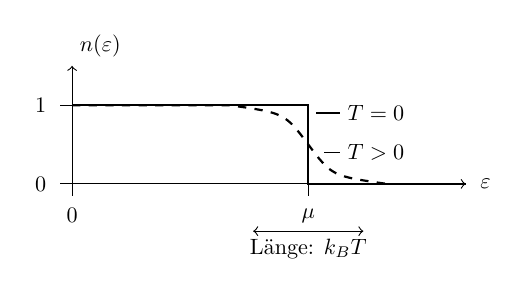
\begin{tikzpicture}[every node/.style={draw=none,fill=none,scale=0.8}]
    \draw[->] (0,-0.15) to (0,1.5);
    \draw[->] (-0.15,0) to (5,0);
    \node[anchor=west] at (0,1.75) {$n(\varepsilon)$};
    \node at (5.25,0) {$\varepsilon$};
    \node at (-0.4,0) {$0$};
    \node at (0,-0.4) {$0$};
    \draw (0,1) to (-0.15,1);
    \node at (-0.4,1) {$1$};
    \draw (3,0) to (3,-0.15);
    \node at (3,-0.4) {$\mu$};
    \draw[thick] (0,1) to (3,1) to (3,0) to (5,0);
    \draw[thick,dashed] (0,1) to (2,1) ..controls (2.7,0.9) .. (3,0.5) .. controls (3.3,0.1) .. (4,0)  (5,0);
    \draw (3.1,0.9) to (3.4,0.9);
    \node[anchor = west] at (3.4,0.9) {$T=0$};
    \draw (3.2,0.4) to (3.4,0.4);
    \node[anchor = west] at (3.4,0.4) {$T>0$};
    \draw[<->] (2.3,-0.6) to (3.7,-0.6);
    \node[anchor = north] at (3,-0.6) {Länge: $k_B T$};
  \end{tikzpicture}
\end{figure}
\begin{tabbing}
\hspace{4em} \= \hspace{4em} \= \kill
Makroskopische Größen wie $N = \int\limits_0^{\infty}\rho(\varepsilon)n(\varepsilon)\dd{\varepsilon}$ oder $E = \int\limits_0^{\infty}\rho(\varepsilon)\varepsilon n(\varepsilon)\dd{\varepsilon}$ sind von der Form\\
$I = \int\limits_0^{\infty} f(\varepsilon) n(\varepsilon) \dd{\varepsilon}$, $I = \int\limits_0^{\mu}f(\varepsilon)\dd{\varepsilon} + \underbrace{\int\limits_0^{\infty}f(\varepsilon)\left(n(\varepsilon) - \Theta(\mu - \varepsilon)\right)\dd{\varepsilon}}_{I'}$
\end{tabbing}
\begin{figure}[H]
  \centering
  \begin{tikzpicture}[every node/.style={draw=none,fill=none,scale=0.8}]
    \draw[->] (0,-0.15) to (0,1.15);
    \draw[->] (-0.15,0) to (5,0);
    \node[anchor= west] at (0,1.4) {$\Theta(\mu -\varepsilon)$};
    \node at (5.25,0) {$\varepsilon$};
    \node at (0,-0.4) {$0$};
    \node at (-0.4,0) {$0$};
    \draw (0,1) to (-0.15,1);
    \node at (-0.4,1) {$1$};
    \draw (3,0) to (3,-0.15);
    \node at (3,-0.4) {$\mu$};
    \draw[thick] (0,1) to (3,1) to (3,0) to (5,0);
  \end{tikzpicture}
  \quad
  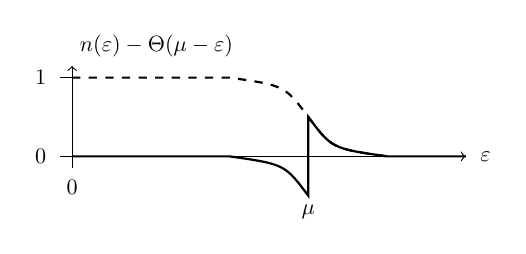
\begin{tikzpicture}[every node/.style={draw=none,fill=none,scale=0.8}]
    \draw[->] (0,-0.15) to (0,1.15);
    \draw[->] (-0.15,0) to (5,0);
    \node[anchor= west] at (0,1.4) {$n(\varepsilon) - \Theta(\mu -\varepsilon)$};
    \node at (5.25,0) {$\varepsilon$};
    \node at (0,-0.4) {$0$};
    \node at (-0.4,0) {$0$};
    \draw (0,1) to (-0.15,1);
    \node at (-0.4,1) {$1$};
    \draw (3,0) to (3,-0.15);
    \node at (3,-0.7) {$\mu$};
    \draw[thick,dashed] (0,1) to (2,1) ..controls (2.7,0.9) .. (3,0.5) .. controls (3.3,0.1) .. (4,0)  (5,0);
    \draw[thick] (0,0) to (2,0) .. controls (2.7,-0.1) .. (3,-0.5) to (3,0.5) .. controls (3.3,0.1) .. (4,0) to (5,0);
  \end{tikzpicture}
\end{figure}
\begin{tabbing}
\hspace{4em} \= \hspace{4em} \= \kill
\underline{Sommerfeld-Entwicklung} (nutze aus, dass der Integrand von I' nur bei $\varepsilon\approx\mu$ ungleich  $0$):\\
$I' \approx \int\limits_{-\infty}^{\infty}\dd{\varepsilon} \sum\limits_{m = 0}^{\infty} \frac{f^{(m)}(\mu)}{m!}(\varepsilon-\mu)^m \left(n(\varepsilon) - \Theta(\mu - \varepsilon)\right) = \sum\limits_{m = 0}^{\infty}\frac{f^{(m)}(\mu)}{m!}(k_B T)^{m+1}\int\limits_{-\infty}^{\infty}x^m\underbrace{\left(\frac{1}{e^x + 1}-\Theta(-x)\right)}_{\text{antisymmetrisch in x}}\dd{x}$\\
Substitution: $x=\beta(\varepsilon-\mu)$ Nur ungerade $m$ tragen bei.\\
$I' \approx 2 f'(\mu)(k_B T)^2 \underbrace{\int\limits_0^{\infty}x\left(\frac{1}{e^x +1}-\Theta(-x)\right)\dd{x}}_{\frac{\pi^2}{12}} + \frac{1}{3} f'''(\mu) (k_B T)^4 \underbrace{\int\limits_0^{\infty} x^3 \left(\frac{1}{e^x +1}-\Theta(-x)\right)\dd{x}}_{\frac{7\pi^4}{120}}$\\
$\rightarrow$\> $I = \int\limits_0^{\mu}f(\varepsilon) \dd{\varepsilon} + \frac{\pi^2}{6}(k_B T)^2 f'(\mu) + \frac{7\pi^4}{360}(k_B T)^4) f'''(\mu) +\dots = I_0 + I_1 + I_3 + \dots$\\
(Anmerkung: Dies ist keine Taylorreihe, sondern eine asymptotische Entwicklung,\\ das heißt für feste Ordnung $m$ und $T\to 0$ geht $I_0 + \dots + I_m - I \to 0$ schneller als $T^m$,\\ aber die Reihe konvergiert nicht für festes $T$ und $m\to \infty$.)\\
\underline{Anwendung auf Teilchenzahl}:\\
$N$\> $= \int\limits_0^{\infty} \rho(\varepsilon) n(\varepsilon) \dd{\varepsilon}$\\
\> $= \int\limits_0^{\mu} \rho(\varepsilon)\dd{\varepsilon} + \frac{\pi^2}{6} (k_B T)^2 \rho'(\mu) + \mathcal{O}\left(T^4\right)$\\
\> $= \frac{g V}{(2 \pi)^2} \left(\frac{2 m}{\hbar^3}\right)^{\frac{3}{2}}\left(\frac{\mu^{3/2}}{3/2} + \frac{\pi^2}{6} (k_B T)^2\cdot \frac{1}{2\mu^{1/2}} + \mathcal{O}\left(T^4\right)\right)$\\
$\rightarrow$\> $\varepsilon_F^{3/2} = \mu^{\frac{3}{2}} \cdot \left(1 + \frac{\pi^2}{8}\left(\frac{k_B T}{\mu}\right)^2 + \mathcal{O}\left(T^4\right)\right)$\\
Für $T\to 0$: $\mu\to \varepsilon_F$, $\varepsilon_F \approx \mu\left(1 + \frac{\pi^2}{6}\left(\frac{k_B T}{\varepsilon_F}\right)^2\right)^{\frac{2}{3}} \approx \mu \left(1 + \frac{2}{3}\frac{\pi^2}{8}\left(\frac{k_B T}{\varepsilon_F}\right)^2\right)$\\
$\rightarrow$\> \fbox{$\mu \approx \varepsilon_F\cdot\left[1-\frac{2}{3}\frac{\pi^2}{8}\left(\frac{k_B T}{\varepsilon_F}\right)^2\right]$}
\end{tabbing}
\begin{figure}[H]
  \centering
  \begin{tikzpicture}[every node/.style={draw=none,fill=none,scale=0.8},domain=0:4]
    \draw[->] (-0.15,0) to (5.25,0);
    \draw[->] (0,-1) to (0,1.25);
    \node at (0,1.5) {$\mu$};
    \node at (5.5,0) {$T$};
    \draw (0,1) to (-0.15,1);
    \node at (-0.4,0) {$0$};
    \node at (-0.4,1) {$\varepsilon_F$};
    \draw[dashed] (0,1) to (5.25,1);
    \draw[thick] plot (\x,{1-\x^2*0.1});
  \end{tikzpicture}
\end{figure}
\begin{tabbing}
\hspace{4em} \= \hspace{4em} \= \kill
Bei hohen $T$ klassisch; $\mu = k_B T \ln\left(\frac{N\Lambda^3}{g V}\right) <0$\\
\underline{Anwendung auf Energie}:\\
$E \stackrel[T\to 0]{}{\approx} \int\limits_0^{\mu} \rho(\varepsilon)\varepsilon \dd{\varepsilon} + \frac{\pi^2}{6} \left. (\rho(\varepsilon)\varepsilon)'\right|{\mu} (k_B T)^2 = \frac{g V}{(2\pi)^2)}\left(\frac{2 m}{\hbar^2}\right)^{\frac{3}{2}}\left(\frac{\mu^{5/2}}{5/2} + \frac{\pi^2}{6}\cdot\frac{3}{2}\mu^{\frac{1}{2}}\cdot(k_B T)^2\right)$\\
Mit Näherung für $\mu(T\to 0)$ (siehe oben): $\mu^{\frac{5}{2}} = \varepsilon_F^{5/2} \left[1-\frac{5}{3}\frac{\pi^2}{6}\left(\frac{k_BT}{\varepsilon_F}\right)^2\right]$\\
$E \approx \frac{3}{2} N \cdot \varepsilon_F^{-3/2}\cdot\left \lbrace \frac{5}{2} \varepsilon_F^{-5/2} \left[ 1-\frac{5}{2} \frac{\pi^2}{6} \left(\frac{k_B T}{\varepsilon_F}\right)^2\right] + \frac{\pi^4}{4}\varepsilon_F^{1/2}(k_B T)^2\right\rbrace$\\
$E\approx \frac{3}{5} N \varepsilon_F \cdot \left[1+\frac{5}{12}\pi^2\left(\frac{k_B T}{\varepsilon_F}\right)^2\right]$\\
$\rightarrow$\> \underline{Wärmekapazität} $C_V  =\left(\frac{\partial E}{\partial T}\right)_{V,N} = \frac{\pi^2}{2} N k_B\cdot \frac{k_B T}{\varepsilon_F}$ oder \fbox{$C_V = \frac{\pi^2}{2} N k_B \frac{T}{T_F}$} (bei $T\to 0$)\\
mit Fermi-Temperatur $T_F = \frac{\varepsilon_F}{k_B}$. Zum Beispiel Elektronen in Cu: 82 000\textbf{K}, Au: 64 000 \textbf{K}.
\end{tabbing}
\begin{figure}[H]
  \centering
  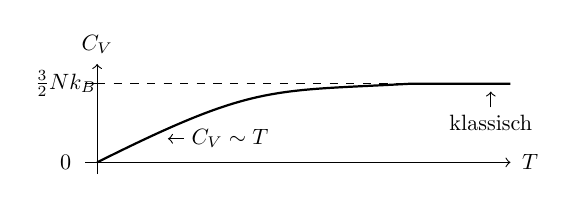
\begin{tikzpicture}[every node/.style={draw=none,fill=none,scale=0.8},domain=0:4]
    \draw[->] (-0.15,0) to (5.25,0);
    \draw[->] (0,-0.15) to (0,1.25);
    \node at (0,1.5) {$C_V$};
    \node at (5.5,0) {$T$};
    \draw (0,1) to (-0.15,1);
    \node at (-0.4,0) {$0$};
    \node at (-0.4,1) {$\frac{3}{2}N k_B$};
    \draw[dashed] (0,1) to (5.25,1);
    \draw[thick] (0,0) .. controls (2,1) and (2.2,0.9) .. (4,1) to (5.25,1);
    \draw[->] (5,0.7) to (5,0.9);
    \node[anchor=north] at (5,0.7) {klassisch};
    \draw[->] (1.1,0.3) to (0.9,0.3);
    \node[anchor=west] at (1.1,0.3) {$C_V \sim T$};
  \end{tikzpicture}
\end{figure}
\begin{tabbing}
\hspace{4em} \= \hspace{4em} \= \kill
Reales Metall bei $T\to 0$: $C_V = A T + B T^3$\\
Wobei $A T$: Elektronen und $B T^3$: Gitterschwingungen (Phononen)\\
Fermi-Gas dient als einfaches Modell für Metallelektronen oder auch Nukleonen im Atomkern oder\\
Neutronensterne. Beispiel $^3$He: $T_F \sim 1\textbf{K}$.
\end{tabbing}


\subsection{Entartetes Bose-Gas}
\begin{tabbing}
\hspace{4em} \= \hspace{4em} \= \kill
Betrachte Gas aus bosonischen Atomen, Einteilchenenergien $\varepsilon = \frac{\vec{p}^2}{2 m}$, $\varepsilon = 0, \dots, \infty$.\\
$\rightarrow$\> Es muss gelten $\mu < 0$, damit $Z = \sum\limits_{n = 0}^{\infty} e^{\beta n(\mu - \varepsilon)} < \infty$.\\
Bei $T = 0$: Alle $N$ Teilchen im Grundzustand $\varepsilon_0 = 0$\\
\> $N = \frac{1}{e^{\beta (\varepsilon_0 - \mu)}} = \frac{1}{e^{-\beta\mu} - 1}$ $\rightarrow$ $e^{-\beta \mu} = \frac{1}{N} +1$\\
$\rightarrow$\> $\mu = - k_B  T \ln\left(1 + \frac{1}{N}\right) \approx -\frac{k_B T}{N} = 0$ für $N \gg 1$\\
Große Temperaturen: klassisches ideales Gas, $\mu = k_B T \ln\left(\frac{N \Lambda^3}{g V}\right)$\\
Ist das Verhalten bei $T\to 0$ mit dem Zustandsdichte-Formalismus beschreibbar?\\ Welche Teilchenzahl $N_C$ gehört zu $\mu = 0$?\\
$\rho(\varepsilon) 0 \frac{g V}{(2\pi)^2} \left(\frac{2 m}{\hbar^2}\right)^{\frac{3}{2}}\varepsilon^{\frac{1}{2}}$, $N = \sum\limits_j \frac{1}{e^{\beta (\varepsilon_j -\mu)}} = \int\limits_0^{\infty}\frac{\rho(\varepsilon)}{e^{\beta(\varepsilon - \mu)}- 1 }\dd{\varepsilon}$\\
$N_C = N(\mu = 0) = \int\limits_0^{\infty} \frac{\rho(\varepsilon)}{e^{\beta\varepsilon}-1}\dd{\varepsilon} = \frac{g V}{(2\pi)^2} \underbrace{\left(\frac{2 m}{\hbar^2}\right)^{\frac{3}{2}} (k_B T)^{\frac{3}{2}}}_{(2\pi)^3\frac{1}{\pi^{3/2}}\Lambda^{-3}} \int\limits_0^{\infty} \frac{x^{1/2}}{e^x - 1}\dd{x}$\\
Es gilt \fbox{$\int\limits_0^{\infty}  \frac{x^{\nu -1}}{e^x - 1}\dd{x} = \Gamma(\nu)\zeta(\nu)$}\\
mit: \> \underline{Gammafunktion} $\Gamma(\nu) = \int\limits_0^{\infty} e^{-t} t^{\nu -1}\dd{t}$,\\
\> \underline{Riemannsche $\zeta$-Funktion} $\zeta(\nu) = \sum\limits_{k = 1}^{\infty}\frac{1}{k^{\nu}}$\\
$\rightarrow$\> $\int\limits_0^{\infty} \frac{x^{1/2}}{e^x-1} \dd{x} = \Gamma\left(\frac{3}{2}\right) \zeta\left(\frac{3}{2}\right) = \frac{\sqrt{\pi}}{2}\cdot\underbrace{\left(1 + \frac{1}{2^{3/2}} + \frac{1}{3^{3/2}} + \dots\right)}_{2.612}$\\
$\rightarrow$\> \fbox{$N_C = g V \Lambda^{-3} \cdot 2.612$}\quad $\Lambda = \frac{h}{\sqrt{2\pi  m k_B T}}$\\
$\rightarrow$\> Es gibt eine \underline{kritische Dichte} $\frac{N_C}{V}$, bei der $\mu = 0$ erreicht wird.\\
Bei gegebener Dichte $\frac{N}{V}$ gibt es eine \underline{kritische Temperatur}\\
$T_C = \frac{1}{k_B} \left(\frac{N/V}{g\cdot 2.612}\right)^\frac{2}{3}\cdot\frac{2\pi \hbar^2}{m}$, wo $\mu = 0$
\end{tabbing}
\begin{figure}[H]
  \centering
  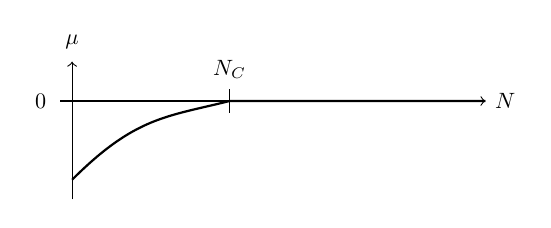
\begin{tikzpicture}[every node/.style={draw=none,fill=none,scale=0.8},domain=0:4]
    \draw[->] (-0.15,0) to (5.25,0);
    \draw[->] (0,-1.25) to (0,0.5);
    \node at (0,0.75) {$\mu$};
    \node at (5.5,0) {$N$};
    \node at (-0.4,0) {$0$};
    \draw[thick] (0,-1) .. controls (0.8,-0.2) and (1.2,-0.2) .. (2,0) to (5.25,0);
    \draw (2,-0.15) to (2,0.15);
    \node at (2,0.4) {$N_C$};
  \end{tikzpicture}
  \quad
  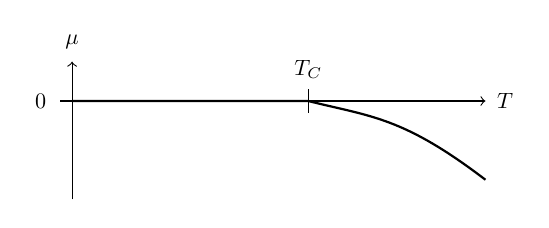
\begin{tikzpicture}[every node/.style={draw=none,fill=none,scale=0.8},domain=0:4]
    \draw[->] (-0.15,0) to (5.25,0);
    \draw[->] (0,-1.25) to (0,0.5);
    \node at (0,0.75) {$\mu$};
    \node at (5.5,0) {$T$};
    \node at (-0.4,0) {$0$};
    \draw[thick] (0,0) to (3,0) .. controls (3.8,-0.2) and (4.2,-0.2) ..  (5.25,-1);
    \draw (3,-0.15) to (3,0.15);
    \node at (3,0.4) {$T_C$};
  \end{tikzpicture}
\end{figure}
\begin{tabbing}
\hspace{4em} \= \hspace{4em} \= \kill
Scheinbar kann die Teilchenanzahl nicht über $N_C$ hinaus erhöht werden, da sonst $\mu$\\ in $N = \int\limits_0^{\infty} \frac{\rho(\varepsilon)}{e^{\beta(\varepsilon-\mu)}-1} \dd{\varepsilon}$ keinen erlaubten Wert annehmen kann.\\
\underline{Lösung}: Integralnäherung versagt; Zustand $\vec{p} = 0$ muss seperat behandelt werden;\\ makroskopische Besetzung in $\varepsilon_0 = 0$.\\
$\rightarrow$\> $N = \underbrace{\frac{1}{e^{-\beta\mu} - 1}}_{N_0} + \underbrace{\int\limits_0^{\infty}\frac{\rho(\varepsilon)}{e^{\beta(\varepsilon - \mu)} - 1} \dd{\varepsilon}}_{N^{*}}$\\
Wobei $N_0 = $ Zahl der Teilchen im Grundzustand, $N^{*} = $ Zahl der Teilchen in angeregten Zuständen\\
Für feste Teilchenzahl $N$:\\
\> $T < T_C$: $\mu = 0$, $N^{*} = \int\limits_0^{\infty}\frac{\rho(\varepsilon)}{e^{\beta(\varepsilon - \mu)} - 1} \dd{\varepsilon} = \frac{g V}{\Lambda^3}\cdot 2.612 = \text{const.}\cdot T^{\frac{3}{2}}$\\
\> $T > T_C$: $\mu < 0$, $N^{*} = N$\\
$\rightarrow$\> $N^{*} = N\cdot \left(\frac{T}{T_C}\right)^{\frac{3}{2}}$ für $T < T_C$, $N_0 = N \cdot \left(1-\left(\frac{T}{T_C}\right)^{\frac{3}{2}}\right)$ für $T < T_C$.\\
\end{tabbing}
\begin{figure}[H]
  \centering
  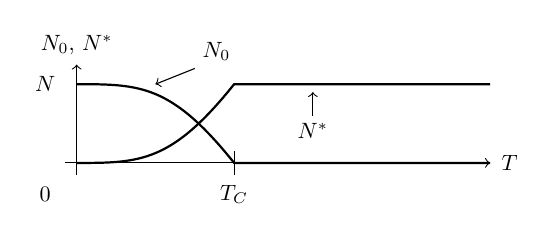
\begin{tikzpicture}[every node/.style={draw=none,fill=none,scale=0.8},domain=0:4]
    \draw[->] (-0.15,0) to (5.25,0);
    \draw[->] (0,-0.15) to (0,1.25);
    \node at (0,1.5) {$N_0$, $N^{*}$};
    \node at (5.5,0) {$T$};
    \node at (-0.4,-0.4) {$0$};
    \node at (-0.4,1) {$N$};
    \draw[thick] (0,0) .. controls (0.8,0) and (1.2,0) ..  (2,1) to (5.25,1);
    \draw[thick] (0,1) .. controls (0.8,1) and (1.2,1) ..  (2,0) to (5.25,0);
    \draw (2,-0.15) to (2,0.15);
    \node at (2,-0.4) {$T_C$};
    \draw[->] (1.5,1.2) to (1,1);
    \node[anchor=south west] at (1.5,1.2) {$N_0$};
    \draw[->] (3,0.6) to (3,0.9);
    \node[anchor=north] at (3,0.6) {$N^{*}$};

  \end{tikzpicture}

\end{figure}
\begin{tabbing}
\hspace{4em} \= \hspace{4em} \= \kill
Die makroskopische Besetzung des Grundzustandes bei $T < T_C$ nennt man\\
\underline{Bose-Einstein-Kondensation} (BEC).\\
\underline{Innere Energie}:\\
$T< T_C$:\> $\mu = 0$, $E = \int\limits_0^{\infty} \frac{\rho(\varepsilon)\varepsilon}{e^{\beta\varepsilon} - 1}\dd{\varepsilon}$ (kein Beitrag des Grundzustands wegen $\varepsilon_0 = 0$)\\
$\rightarrow$ $E$\> $= \frac{g V}{(2\pi)^2}\left(\frac{2 m}{\hbar^2}\right)^{\frac{3}{2}} (k_B T)^{\frac{5}{2}}
\underbrace{ \int\limits_0^{\infty}\frac{x^{3/2}}{e^x-1}\dd{x}}_{\Gamma\left(\frac{5}{2}\right)\zeta\left(\frac{5}{2}\right)}$\\
\> $=\underbrace{\frac{g V}{(2\pi)^2}\left(\frac{2 m k_B T}{\hbar^2}\right)^{\frac{3}{2}}\Gamma\left(\frac{3}{2}\right)\zeta\left(\frac{3}{2}\right)}_{N^{*}} k_B T\underbrace{\frac{\gamma(5/2)\zeta(5/2)}{\gamma(3/2)\zeta(3/2)}}_{0.77}$\\
$\rightarrow$\> \fbox{$E = 0.77\cdot N k_B T \left(\frac{T}{T_C}\right)^{\frac{3}{2}}$}\\
$T > T_C$:\> $E = \int\limits_0^{\infty}\frac{\rho(\varepsilon)\varepsilon}{e^{\beta (\varepsilon - \mu)} -1}\dd{\varepsilon} = \frac{g V}{(2\pi)^2}\left(\frac{2 m}{\hbar^2}\right)^{\frac{3}{2}}(k_B T)^{\frac{5}{2}}\underbrace{\int\limits_0^{\infty}\frac{x^{3/2}}{e^xz^{-1} -1}\dd{x}}_{\Gamma\left(\frac{5}{2}\right)g_{\frac{5}{2}}(z)}$\\
\> mit $z:= e^{\beta\mu}$, $g_{\nu}(z) := \frac{1}{\Gamma(\nu)}\int\limits_0^{\infty}\frac{x^{\nu -1}}{e^xz^{-1} -1}\dd{x}$ (\glqq\underline{verallgemeinerte $\zeta$-Funktion}\grqq)\\
$\rightarrow$\> $E = \frac{g V}{(2\pi)^2)}\left(\frac{2 m}{\hbar^2}\right)^{\frac{3}{2}}(k_B T_C)^{\frac{3}{2}}\left(\frac{T}{T_C}\right)^{\frac{3}{2}}\Gamma\left(\frac{3}{2}\right)\zeta\left(\frac{3}{2}\right)k_B T \frac{\Gamma(5/2)g_{5/2}(z)}{\Gamma(3/2)\zeta(3/2)}$\\
\> $E = N k_B T \left(\frac{T}{T_C}\right)^{\frac{3}{2}}\cdot 0.574 g_{\frac{5}{2}}(z)$\\
(Dabei ist $z$ zu bestimmen aus $N = N\cdot \left(\frac{T}{T_C}\right)^{\frac{3}{2}}\frac{g_{3/2}(z)}{\zeta(3/2)}$, das heißt $2.612\cdot \left(\frac{T}{T_C}\right)^{\frac{3}{2}} = g_{\frac{3}{2}}(z)$.)\\
\underline{Druck}:\\
$E = \frac{3}{2} p V$ $\rightarrow$ $p = \frac{2 E}{3 V}$\\
$T < T_C$:\> $p = \frac{\Gamma(5/2)\zeta(5/2)}{\Gamma(3/2)\zeta(3/2)}\frac{2}{3}\frac{N}{V} k_B T \left(\frac{T}{T_C}\right)^{\frac{3}{2}}$, $T_C = \frac{1}{k_B}\frac{(N/V)^{2/3}}{(g\cdot \zeta(3/2))^{2/3}}\frac{2\pi \hbar^2}{m}$\\
\> $T_C^{\frac{3}{2}} = \left(\frac{2\pi\hbar^2}{m k_B}\right)^{\frac{3}{2}}\frac{N/V}{g\cdot \zeta(3/2)}$,
$\Lambda^3 = \left(\frac{4\pi^2\hbar^2}{2\pi m k_B T}\right)^{\frac{3}{2}} = \left(\frac{2\pi\hbar^2}{m k_B T}\right)^{\frac{3}{2}}$\\
\> $p = \zeta\left(\frac{5}{2}\right)\cdot g\cdot k_B T\cdot \Lambda^{-3}$\\
\> $p = 1.341 \frac{g k_B T}{\Lambda^3}$, $p \stackrel[T\to o]{}{\longrightarrow}0$\\
\> (Eigentlich: $\varepsilon_0 = \frac{\hbar^2}{2 m}\left(\frac{\pi}{L}\right)^2$ und $p = -\frac{\partial E_0}{\partial V}$ mit $E_0 = N \frac{\hbar^2}{2 m} \pi^2 V^{-\frac{2}{3}}$)\\
$T > T_C$:\> $p = g_{\frac{5}{2}}(z)\cdot \frac{g k_B T}{\Lambda^3}$\\
\underline{Wärmekapazität}:\\
$C_V = \left(\frac{\partial E}{\partial T}\right)_{N,V}$\\
$T < T_C$:\> $C_V = 1.923\cdot N k_B \left(\frac{T}{T_C}\right)^{\frac{3}{2}} = 1.923 N^{*} k_B$\\
$T > T_C$:\> $C_V = \frac{\partial}{\partial T}\left(\frac{3}{2}g_{\frac{5}{2}}(z)\frac{g k_B T V}{\Lambda^3}\right)_{N,V} = \frac{15}{4}g_{\frac{5}{2}}(z)\frac{g k_B V}{\Lambda^3} + \frac{3}{2}g'_{\frac{5}{2}}(z)\frac{\partial z}{\partial T}\frac{g k_B T V}{\Lambda^3}$\\
\> Man findet: $C_V = \frac{15}{4} g_{\frac{5}{2}}(z)\frac{g k_B V}{\Lambda^3} - \frac{9}{4} N k_B \frac{g_{3/2}(z)}{g_{1/2}(z)}$\\
\end{tabbing}
\begin{figure}[H]
  \centering
  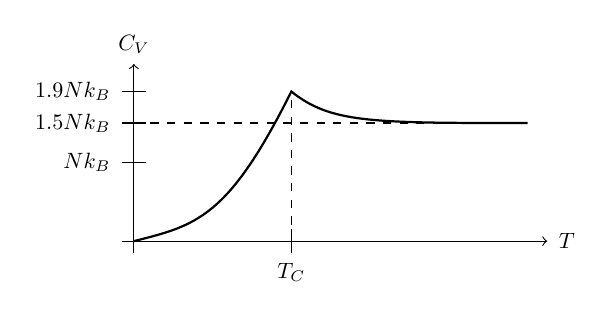
\begin{tikzpicture}[every node/.style={draw=none,fill=none,scale=0.8},domain=0:4]
    \draw[->] (-0.15,0) to (5.25,0);
    \draw[->] (0,-0.15) to (0,2.25);
    \node at (0,2.5) {$C_V$};
    \node at (5.5,0) {$T$};
    \draw (-0.15,1) to (0.15,1);
    \draw (-0.15,1.9) to (0.15,1.9);
    \draw (-0.15,1.5) to (0.15,1.5);
    \node[anchor=east] at (-0.2,1) {$N k_B$};
    \node[anchor=east] at (-0.2,1.5) {$1.5 N k_B$};
    \node[anchor=east] at (-0.2,1.9) {$1.9 N k_B$};
    \draw (2,-0.15) to (2,0.15);
    \node at (2,-0.4) {$T_C$};
    \draw[dashed] (2,0) to (2,1.9);
    \draw[dashed] (0,1.5) to (5,1.5);
    \draw[thick] (0,0) .. controls (0.8,0.2) and (1.2,0.3) ..  (2,1.9) .. controls (2.5,1.5) and (3,1.5) .. (5,1.5);
  \end{tikzpicture}
\end{figure}
\begin{tabbing}
\hspace{4em} \= \hspace{4em} \= \kill
\underline{Geschichte}:\\
1924:\> Vorhersage der Bose-Einstein-Kondensate (Bose, Einstein)\\
1938:\> Vermutung, dass BEC mit Suprafluidität in $^4$He zusammenhängt. (Allerdings kann flüssiges\\\> He aufgrund der Wechselwirkungen nicht als ideales Quantengas betrachtet werden.)\\
1995:\> Erstes gasartiges BEC (Cornell, Wiemann), $\sim 2000$ Rb-Atome bei $170 \text{n}\textbf{K}$\\
1995:\> BEC mit $\sim 500 000$ Na-Atomen (Ketterle)\\
2001:\> Nobelpreis Cornell, Wiemann, Ketterle\\
\end{tabbing}


\subsection{Photonengas}
\begin{tabbing}
\hspace{4em} \= \hspace{4em} \= \kill
-- Photon-Photon-Wechselwirkung extrem schwach\\\>$\rightarrow$ gutes ideales Gas!\\
-- Zum Erreichen eines Gleichgewichts ist Wechselwirkung mit Umgebung notwendig.\\ \>$\rightarrow$ Betrachte Photonen in einem Hohlraum mit Volumen $V$, Temperatur $T$\\
-- \underline{Schwarzer Körper} (perfekt absorbierend) strahlt wie Loch eines Hohlraums.\\
\>$\rightarrow$ Schwarzkörperstrahlung, Hohlraumstrahlung\\
-- Empirisch: Strahlungsspektrum hängt nur von $T$ ab.\\
\> 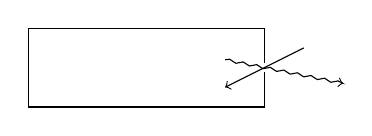
\begin{tikzpicture}[every node/.style={draw=none,fill=none,scale=0.8}]
\draw (3,0.56) to (3,1) to (0,1) to (0,0) to (3,0) to (3,0.44);
\draw[<-] (2.5,0.25) to (3.5,0.75);
\draw[->,decoration={snake,amplitude=0.5,segment length=5},decorate] (2.5,0.6) to (4,0.3);
\end{tikzpicture} charakteristisch für T$\rightarrow$ Ohrthermometer\\
-- Teilchenzahl kann nicht kontrolliert werden (jedenfalls nicht unabhängig von der Energie)\\\> $\rightarrow$ Rechnung wie im kanonischen beziehungsweise großkanonischen Ensemble mit $\mu = 0$.\\
\underline{Photonenstatistik}:\\
Zustandssumme $Z = \prod\limits_j Z_j$ mit $Z_j = \sum\limits_n e^{-\beta n \varepsilon_j} =$ Zustandssumme der Mode $j = (\vec{p},\lambda)$\\
Mode angegeben durch Impuls $\vec{p}$, Polarisation $\lambda = \pm 1$ (links-/ rechtszirkular)\\
Boltzmannfaktoren $e^{-\beta n \varepsilon_j}$ $\rightarrow$ mittlere Photonenanzahl $\langle n_j \rangle = \frac{1}{e^{\beta\varepsilon_j} - 1}$\\
Dispersionsrelation: $\varepsilon = c |\vec{p}|$ (mit $\varepsilon = \hbar \omega$, $\vec{p} = \hbar \vec{k}$)\\
Zustandsdichte $\rho$ als Funktion der (Kreisfrequenz): $\rho(\omega)\dd{\omega} = 2\cdot \frac{4\pi \vec{p}^2 V}{h^3}\dd{p}$\\
$|\vec{p}| = \frac{\hbar \omega}{c}$\> $\rightarrow$\> $\rho(\omega) = \frac{8\pi}{(2\pi c)^3}\omega^2 V = \frac{\omega^2 V}{\pi^2c^3}$\\
\underline{Spektrale Energiedichte } (Energie pro $\dd{\omega}$ und pro Volumen):\\
$u(\omega,T) = \frac{\rho(\omega)}{V}\cdot \hbar \omega \cdot \langle n\rangle$ $\rightarrow$ \fbox{$u(\omega,T) = \frac{\hbar \omega^3}{\pi^2 c^3 \left(e^{\beta\hbar\omega} -1\right)}$} (\underline{Plancksches Strahlungsgesetz})
\end{tabbing}
\begin{figure}[H]
  \centering
  \begin{tikzpicture}[every node/.style={draw=none,fill=none,scale=0.8},domain=-0.15:10]
    \draw[->] (-0.15,0) to (10.25,0);
    \draw[->] (0,-0.15) to (0,2.25);
    \node at (0,2.5) {$u(\omega,T)$};
    \node at (10.5,0) {$\omega$};
    \node at (0,-0.4) {$0$};
    \draw[thick] plot function{x**3/(exp(x)-1)};
  \end{tikzpicture}
\end{figure}
\begin{tabbing}
\hspace{4em} \= \hspace{4em} \= \kill
\uwave{Beispiel}: Hintergrundstrahlung des Universums, $T = 2.73\textbf{K}$.\\
Grenzfälle:\\
a)\> $\hbar \omega \ll k_B T$ (klassischer Grenzfall) $\rightarrow$ $u(\omega, T) = \frac{k_B T \omega^2}{\pi^2 c^3}$ (Rayleigh-Jeans-Gesetz)\\
\> (würde für $\omega\to 0$ zu einer Divergenz führen; \glqq Ultraviolettkatastrophe\grqq )\\
b)\> $\hbar\omega \gg k_B T$ $\rightarrow$ $u(\omega,T) = \frac{\hbar\omega^3}{\pi^2 c^3}e^{-\beta \hbar \omega}$ (Wiensches Gesetz)\\
\underline{Energiedichte}:$\frac{E}{V} = \int\limits_0^{\infty} u \dd{\omega} = \frac{1}{\pi^2 c^3\hbar^3} (k_B T)^4 \underbrace{\int\limits_0^{\infty}\frac{x^3}{e^x-1}\dd{x}}_{\Gamma(4)\zeta(4) = \frac{\pi^4}{15}}$\\
$\rightarrow$\> \fbox{$\frac{E}{V} = \frac{\pi^2}{15 \hbar^3 c^3} (k_B T)^4$} (\underline{Stefan-Boltzmann-Gesetz})\\
Umrechnung in abgestrahlte Energie pro Fläche und Zeit:\\
\> \fbox{$I = \frac{c}{4}\cdot \frac{E}{V} = \sigma  T^4$} mit Stefan-Boltzmann-Konstante $\sigma = \frac{k_B^4\pi^2}{60 \hbar^3c^2}$.\\
\underline{Wärmekapazität}: $C_V = \left(\frac{\partial E}{\partial T}\right)_V = \frac{16\sigma}{c} V T^3$.\\
\underline{Freie Energie} (beziehungsweise großkanonnisches Potential, da $\mu = 0$):\\
\> $F = - k_B T \ln Z = - k_B T \sum\limits_j \ln Z_j = k_B T \int\limits_0^{\infty} \ln\left(1-e^{-\beta\hbar\omega}\right)\rho(\omega)\dd{\omega}$\\
\>   $= \frac{k_B T V}{\pi^2 c^3}\left\{\left[\frac{\omega^3}{3}\ln\left(1-e^{-\beta\hbar\omega}\right)\right]_0^{\infty} - \frac{\beta\hbar}{3}\int\limits_0^{\infty}\frac{\omega^3 e^{-\beta\hbar\omega}}{1 - e^{-\beta\hbar\omega}}\dd{\omega}\right\}$\\
$\rightarrow$\> $F = -\frac{E}{3} = -\frac{4}{3}\frac{\sigma}{c}\cdot V T^4$
\end{tabbing}
